\documentclass[10pt]{beamer}
\usetheme[
%%% options passed to the outer theme
%    progressstyle=movCircCnt,   %either fixedCircCnt, movCircCnt, or corner
%    rotationcw,          % change the rotation direction from counter-clockwise to clockwise
%    shownavsym          % show the navigation symbols
  ]{AAUsimple}
  
% If you want to change the colors of the various elements in the theme, edit and uncomment the following lines
% Change the bar and sidebar colors:
%\setbeamercolor{AAUsimple}{fg=red!20,bg=red}
%\setbeamercolor{sidebar}{bg=red!20}
% Change the color of the structural elements:
%\setbeamercolor{structure}{fg=red}
% Change the frame title text color:
%\setbeamercolor{frametitle}{fg=blue}
% Change the normal text color background:
%\setbeamercolor{normal text}{fg=black,bg=gray!10}
% ... and you can of course change a lot more - see the beamer user manual.

\usepackage[utf8]{inputenc}
\usepackage[english]{babel}
\usepackage[T1]{fontenc}
% Or whatever. Note that the encoding and the font should match. If T1
% does not look nice, try deleting the line with the fontenc.
\usepackage{helvet}
\usepackage{tikz}

% colored hyperlinks
\newcommand{\chref}[2]{%
  \href{#1}{{\usebeamercolor[bg]{AAUsimple}#2}}%
}

\setbeamertemplate{footline}[frame number]

\title{Using Horn Clauses for Analyzing Security Protocols Presentation}

\subtitle{Bruno Blanchet}  % could also be a conference name

\date{\today}

\author{
  Bruno Thalmann\\
  \href{mailto:bthalm11@student.aau.dk}{{\tt bthalm11@student.aau.dk}}
}

% - Give the names in the same order as they appear in the paper.
% - Use the \inst{?} command only if the authors have different
%   affiliation. See the beamer manual for an example

\institute[
%  {\includegraphics[scale=0.2]{aau_segl}}\\ %insert a company, department or university logo
  Dept.\ of Computer Science\\
  Aalborg University\\
  Denmark
] % optional - is placed in the bottom of the sidebar on every slide
{% is placed on the bottom of the title page
  Department of Computer Science\\
  Aalborg University\\
  Denmark
  
  %there must be an empty line above this line - otherwise some unwanted space is added between the university and the country (I do not know why;( )
}

% specify a logo on the titlepage (you can specify additional logos an include them in 
% institute command below
\pgfdeclareimage[height=1.5cm]{titlepagelogo}{AAUgraphics/aau_logo_new} % placed on the title page
%\pgfdeclareimage[height=1.5cm]{titlepagelogo2}{AAUgraphics/aau_logo_new} % placed on the title page
\titlegraphic{% is placed on the bottom of the title page
  \pgfuseimage{titlepagelogo}
%  \hspace{1cm}\pgfuseimage{titlepagelogo2}
}

\begin{document}
% the titlepage
{\aauwavesbg%
\begin{frame}[plain,noframenumbering] % the plain option removes the header from the title page
  \titlepage
\end{frame}}
%%%%%%%%%%%%%%%%

%%%%%%%%%%%%%%%%

\begin{frame}
  \frametitle{Motivation}
   Designing security protocols is difficult:
  \begin{itemize}
  \item Simple authentication - has many considerations
  \item Environment - the attackers capabilities
  \item Manipulating messages, monitoring, crypto attack, timing attacks etc.
  \end{itemize}
  \begin{center}
    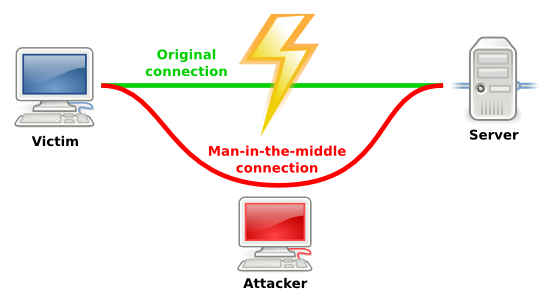
\includegraphics[width=0.5\textwidth]{graphics/man-in-the-middle.png}    
  \end{center}

\end{frame}

\begin{frame}
  \frametitle{ProVerif}
  \begin{itemize}
  \item Check security protocols
  \item Secrecy and authentication
  \item Fully automatic
  \item First order logic
  \item How to use
  \end{itemize}
\end{frame}


\begin{frame}
  \frametitle{Dolev-Yao model}
  \begin{itemize}
  \item Formal model
    \\~\\
  \item Machines exchange messages in form of formal terms
    \\~\\
  \item The attacker can listen, intercept, send and alter messages
  \end{itemize}
\end{frame}

\begin{frame}
  \frametitle{Syntax}
  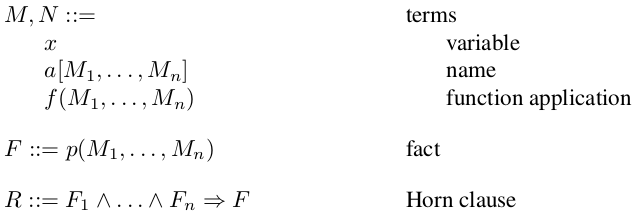
\includegraphics[width=.8\textwidth]{graphics/syntax.png}
\end{frame}


\begin{frame}
  \frametitle{Cryptographic primitives}
  \begin{itemize}
  \item Constructors
    \begin{itemize}
    \item pencrypt
    \item pk
    \item sign
    
    \end{itemize}
    
  \item Destructors
    \begin{itemize}
    \item getmess
    \item checksign
    \item pdecrypt
    \end{itemize}
  \end{itemize}
\end{frame}

\begin{frame}
  \frametitle{Attacker}
  Assumptions about the attacker. The attacker can:
  \begin{itemize}
  \item Intercept all messages.
  \item Compute new messages from the one he has received.
  \item Send messages he can build.
  \item Use all constructors and destructors
  \item Compute new names
  \end{itemize}
\end{frame}

\begin{frame}
  \frametitle{Protocol}
  \begin{itemize}
  \item Computation abilities of the attacker
    \\~\\
  \item Initial knowledge of the attacker
    \\~\\
  \item Messages of the protocol
  \end{itemize}
\end{frame}


\begin{frame}
  \frametitle{Secrecy}
  \begin{itemize}
  \item Listen, intercept, send, alter
  \item Main goal: Can the attacker get secret $s$?
  \item Given the clauses can $attacker(s)$ be derived.
  \item The sequence of this derivation is the attack.
  \end{itemize}
\end{frame}


\begin{frame}
  \frametitle{Handshake protocol example}
  Given two principals: $A$ and $B$
  \\~\\
  Message 1: $A \rightarrow B : \{[k]_{sk_{A}}\}_{pk_{B}}$
  \\~\\
  Message 2: $B \rightarrow A : \{s\}_{k}$
\end{frame}

\begin{frame}
  \frametitle{Handshake protocol example input I}
  Describing the protocol:
  \\~\\
  Computations abilities of the attacker:
  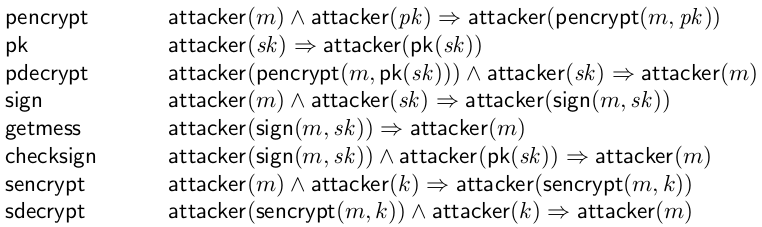
\includegraphics[width=.9\textwidth]{graphics/abilities.png}
  
\end{frame}

\begin{frame}
  \frametitle{Handshake protocol example input II}
  Initial knowledge:
  \begin{itemize}
  \item $attacker(pk(sk_A[]))$
  \item $ attacker(pk(sk_B[]))$
  \end{itemize}
  The protocol:
  \begin{enumerate}
  \item $attacker(pk(x)) \implies attacker(pencrypt(sign(k[pk(x)],sk_A),pk(x)))$
  \item $attacker(pencrypt(sign(y,sk_A[]),pk(sk_B[]))) \implies attacker(sencrypt(s,y))$
  \end{enumerate}
\end{frame}

\begin{frame}
  \frametitle{Handshake protocol example attack}
  $attacker(s)$ is derivable from the clauses given communication between A and B the attack is the following derivation:
  \begin{enumerate}
  \item Fresh name $a[]$ and compute $pk(a[])$
  \item Get and decrypt the first message: $pencrypt(sign(k,sk_A[]),pk(a[]))$ 
  \item The message is than reencrypted under $pk(sk_B[])$ and send to B
  \item B now thinks it is communicating with A and sends: $sencrypt(s,k)$
  \item Since the attacker has k from the first message $sdecrypt$ yields the secret
  \end{enumerate}
\end{frame}


\begin{frame}
  \frametitle{Resolution Algorithm}
  \begin{itemize}
  \item Given a set of Horn clauses can a fact be derived.

  \item The selection function, from clauses to facts
  \item First phase: Transforms the given clauses a new one
  \item Second phase: DFS to determine whether a fact can be derived
  \item Optimizations
  \item Termination
  \end{itemize}
\end{frame}

\begin{frame}
  \frametitle{Experimental results comments}
  \begin{itemize}
  \item Not really any new showed in the paper
  \item Sources on other research groups using ProVerif
  \item Homepage of ProVerif
  \end{itemize}
\end{frame}

\begin{frame}
  \frametitle{Experimental results}
  \begin{center}
    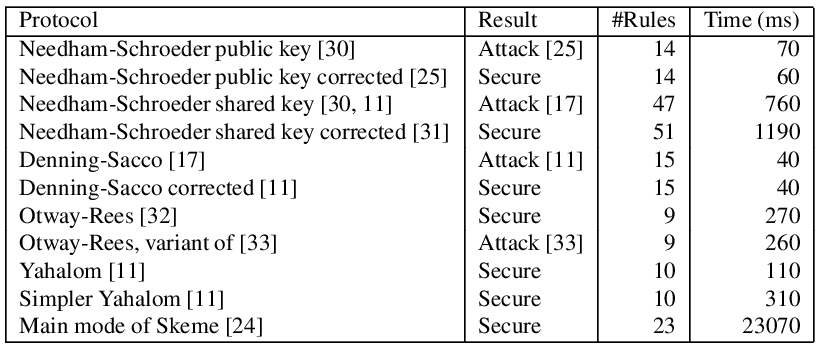
\includegraphics[width=.8\textwidth]{graphics/results.png}
  \end{center}
  From \textit{An Efficient Cryptographic Protocol Verifier Based on Prolog Rules}
\end{frame}

\begin{frame}
  \frametitle{Contribution}
  \begin{itemize}
  \item \textit{An Efficient Cryptographic Protocol Verifier Based on Prolog Rules}
  \item \textit{The NRL Protocol Analyzer: An Overview}
  \item ProVerif: Easy to use, Fast
  \item Describe protocol with horn clauses or applied calculus
  \item Good \textit{``survey''}
  \end{itemize}
\end{frame}


{\aauwavesbg
\begin{frame}[plain,noframenumbering]
  \finalpage{Questions}
\end{frame}}
%%%%%%%%%%%%%%%%

\end{document}
